\documentclass{article}
\usepackage{graphicx}
\graphicspath{{figures/}}
\usepackage{subfigure}
\usepackage{listings}
\usepackage{color} %red, green, blue, yellow, cyan, magenta, black, white
\definecolor{mygreen}{RGB}{28,172,0} % color values Red, Green, Blue
\definecolor{mylilas}{RGB}{170,55,241}

\title{Sections and Chapters}
\author{Gubert Farnsworth}
\date{ ENME 625: Multi-Displinary Optimization \\ 5/12/2017}
 
\begin{document}
 
\maketitle

\newpage
 
\tableofcontents
 
\newpage 
 
\section{Introduction}
 
This is the first section.
 

 
\addcontentsline{toc}{section}{Problems}
\section*{Unconstrained MOGA Problems}
We used this textbook \cite{deb2001multi}

\subsection{ ZDT1} 
Talk about ZDT1 here.  


\begin{align*}
\textrm{Minimize} ~~~~~ f_1(\textbf{x}) &= X_1 \\
\textrm{Maximize} ~~~~ f_2(\textbf{x}) &= g*h \\
\testrm{where} ~~~~~~~~~ g &= 1+\frac{9}{(nvar-1)}.*sum_{i=2}^nvar(X_i) \\
~~~~~~~~~ h &= 1- sqrt{\frac{f_1}{g}} \\
~~~~~~~~~ nvar &= 30 \\
\textrm{subject to} \textbf{X} &= \textbf{X} \leq 1 \\
\textbf{X} &= \textbf{X} \geq 0 \\
\end{align*}


\section{Constrained MOGA Problems}
This is a reference to Azarms constraint paper \cite{kurpati2002constraint}. %This is how references are read from the references.bib file.
 
\subsection{TNK}

Here is figure \ref{fig:TNK}.


\begin{figure}%[tbp]
  \centering
  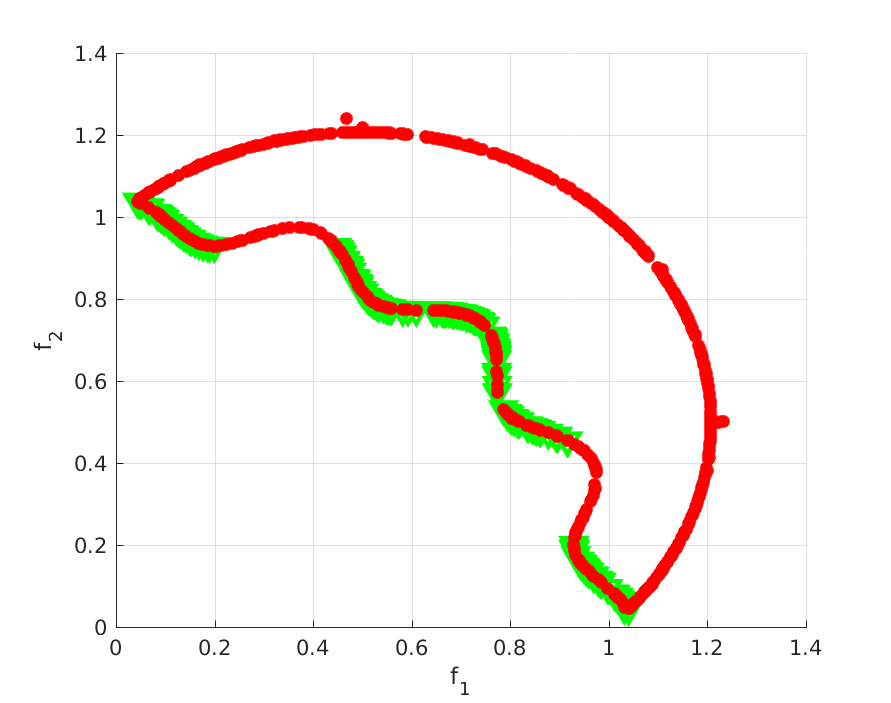
\includegraphics[width=0.50\columnwidth]{5_020_1000.png}
  \caption{ This is TNK for 20 chromosomes and 1000 runs}
  \label{fig:TNK}
\end{figure}
 
\vspace{-0.1in}
\bibliographystyle{IEEEtran}
\bibliography{references.bib}
 
 

\section{Appendix}

%Matlab codes starts here
 

\lstset{language=Matlab,%
    %basicstyle=\color{red},
    breaklines=true,%
    morekeywords={matlab2tikz},
    keywordstyle=\color{blue},%
    morekeywords=[2]{1}, keywordstyle=[2]{\color{black}},
    identifierstyle=\color{black},%
    stringstyle=\color{mylilas},
    commentstyle=\color{mygreen},%
    showstringspaces=false,%without this there will be a symbol in the places where there is a space
    numbers=left,%
    numberstyle={\tiny \color{black}},% size of the numbers
    numbersep=8pt, % this defines how far the numbers are from the text
    emph=[1]{for,end,break},emphstyle=[1]\color{red}, %some words to emphasise
    %emph=[2]{word1,word2}, emphstyle=[2]{style},    
}


\section*{Matlab Code}

\lstinputlisting{MasterCode.m}
\lstinputlisting{fitFCN5.m}


\end{document}
